%%
%%  Project:        Dissertation
%%  File:           $RCSfile$
%%  Version:        $Revision$
%%  Creation date:  Mon March 27, 2000
%%  Last changes:   $Date$
%%  Author:         $Author$
%%                  bauer@vmars.tuwien.ac.at
%%  Contents:       Main LaTeX File
%%
%%  FileID:         $Id$
%%

\documentclass[12pt,a4paper,oneside]{scrreprt}

\usepackage{graphicx}          %includegraphics-command
\usepackage{fancyheadings}
\usepackage{url}
\usepackage[english,germanb]{babel}
\usepackage[latin1]{inputenc}  %support direct writing of German Umlauts
\usepackage{dcolumn}           %decimal column formatting

\newcolumntype{d}[1]{D{.}{.}{#1}}              % decimal formatting in tables
\newcolumntype{C}[1]{@{}>{\centering}p{#1}@{}} % centered columns with fixed width: C{width}

\usepackage{mybakktitlepage}

%%
%% ---------------------------------------------------------------------
%%

\sloppy

\oddsidemargin 1cm \evensidemargin 1cm \topmargin 0pt

\headsep 50pt \textheight 21.4cm \textwidth 14.1cm
\setlength{\parskip}{5pt plus2pt minus2pt}

\renewcommand{\floatpagefraction}{0.9}
\renewcommand{\textfraction}{0.05}
\renewcommand{\topfraction}{1.0}
\renewcommand{\bottomfraction}{1.0}

\setcounter{totalnumber}{5}
\setcounter{bottomnumber}{5}
\setcounter{topnumber}{5}

\setcounter{tocdepth}{2}
\addtolength{\abovecaptionskip}{-10pt}

\newcommand{\eg}{e.\,g., }
\newcommand{\ie}{i.\,e., }
\def\lqq{\lq\lq}
\def\rqq{\rq\rq}
\def\dq#1{\lqq #1\rqq}
\def\dqit#1{\lqq \emph{#1}\rqq}

%%
%% ---------------------------------------------------------------------
%%

%%
%% Acronym definitions
%%
%% This file should be edited by user
%%

\usepackage{acronym}

% Declare acronym using:
%    \newacro{acronym}{expanded name}
% Use Acronym in text:
%    \ac{acronym}

\newacro{GPL}{Gnu Public License}


%%
%% ---------------------------------------------------------------------
%%

\begin{document}

    \pagestyle{empty}
    %%
%% Title
%%
%% This file should be edited by user
%%

\title{embedded operating systems / tinyOS}
\author{Harad Glanzer}
\address{Hardtgasse 25 / 12A, 1190 Wien}
\matrikel{0727156}
\date{September 2011}

\advisorname{Dipl.-Ing Alexander K{\"o}ssler}
\institut{Institut f{\"u}r Technische Informatik}
\instnummer{182}

%%
%% = eof =====================================================================
%%

    \maketitle
    \cleardoublepage

    \pagestyle{plain}
    \pagenumbering{roman}
    \setlength{\parskip}{5pt plus2pt minus2pt}

    \setcounter{page}{1}

%% if thesis is in English language use the following paragraph:
%%
    \selectlanguage{english}
    %%
%% Abstract
%%
%% This file should be edited by user
%%

\renewcommand{\englabstractname}{}
\begin{abstract}
\begin{center}
\parbox{.95\textwidth}
{ \setlength{\parindent}{3ex}
\setlength{\parskip}{0.3\baselineskip}

\noindent 

Subject of this work is to give an introduction to the TinyOS Embedded Operating System, to explain the internal structure of this OS and to present its main components. Additionally, tinyOS is compared to another embedded OS, MicroC/OS-II. Because tinyOS will be used in future lectures at the TU Wien, there is also a chapter about installing tinyOS from scratch. Also, there is a chapter about new tinyOS modules for the bigAVR6 - developementplatform that have been written by me in the course of my project thesis. 


 }
\end{center}
\end{abstract}

%%
%% = eof =====================================================================
%%

    \cleardoublepage
%%

%% if thesis is in German language use the following paragraph:
%
%    \selectlanguage{german}
%    \include{kurzfassung}
%    \cleardoublepage
%
%%
    \setlength{\parskip}{1mm}
    \linespread{0.0}

    \tableofcontents
%    \listoffigures
%    \listoftables
    \linespread{1}
    \clearpage
    \cleardoublepage
    \setlength{\parskip}{5pt plus2pt minus2pt}

    \pagestyle{fancy}
    \renewcommand{\chaptermark}[1]{\markboth{\thechapter\ #1}{}}
    \renewcommand{\sectionmark}[1]{\markright{\thesection\ #1}{}}
    \addtolength{\headheight}{2pt}

    \pagenumbering{arabic}
    \setcounter{page} {1}
    \cleardoublepage
    %%
%% Introduction
%%
%% This file should be edited by user
%%

\chapter{Introduction} \label{chapter:introduction}

This work is about explaining tinyOS. tinyOS is an opensource operating system, designed for use with wireless embedded sensor networks. There are 2 major stable branches, v.1.x and v2.x, which are not compatible to each other. tinyOS 2.x introduced some major improvements, for example the task scheduler was completely redesigned. In it's new version, the whole project us now distributed under the new BSD license too.

Because of tinyOS's component-based architecture, a highlevel programmer does not have to care about microcontroller specifics, as long as the necessary modules are already exisiting. So, implementing new applications or changing exisiting ones is an easy and fast task. There are already existing implementations for a range of popular hardware notes, as for example the mica, iris and teleosa motes.

For developing applications in tinyOS, NesC is used. NesC stands for Network Embedded Systems C, which is very similar to C/C++. Components in NesC are related to objects in C++.

Embedded systems are designed for one or a few specific tasks, perhaps in combination with realtime constraints.
Because embedded systems are often battery powered, one of the main requirements is low power consumption, so that high operation times can be achieved - flexibility is not that important.

This work has to be considered as part of another work, where tinyOS was ported to a new platform, the bigAVR6 development platform. So, a big part of this work handles about the bigAVR6 platform and explains some new written softwaremodules for highlevel-use of this platform's peripherals. It is also explained how to get a running buildenvironment for writing applications or extending the modules for an exisiting platform from scratch.

\section{Motivation and Objectives}

Ultimate goal of this work is to provide an easy-to-use manual for using tinyOS to the reader, so that a buildenvironement can be set up from scratch step-by-step without any necessary previous knowledge. By comparing tinyOS to another embedded operating system - MicroC/OS-II -  the specific characteristics of tinyOS will get much clearer. Finally, by guidung through the selfwritten software modules for the bigAVR6-board, the reader will get familiar with how to practically extend the tinyOS framework by using as much of the preexisting components and how to properly integrate the selfwritten code into tinyOS.

\section{Structure of the Thesis} \label{sec:introduction:structure}

The thesis is structured as follows:

Chapter~\ref{chapter:tinyos} gives a more detailed overview over tinyOS and explains its internals. It also compares tinyOS to another embedded operation system, MicroC/OS-II.

Chapter~\ref{chapter:nesC} gives an introduction to nesC.  

Chapter~\ref{chapter:bigAVR6} introduces the developement platform bigAVR6, for which tinyOS was ported to by the author, and explains the supported devices for this platform. 

Chapter~\ref{chapter:osII} introduces another embedded operation system, named MicroC/OS-II, and compares it's main characteristics to tinyOS.

Chapter~\ref{chapter:buildenv} is a step-by-step howto for setting up a fresh tinyOS - environment.

%Finally, the thesis ends with a conclusion in
%Chapter~\ref{chapter:conclusion} summarizing the key results of the
%presented work and giving an outlook on what can be expected from
%future research in this area.

%%
%% = eof =====================================================================
%%

    \cleardoublepage
    %%
%%
%% This file should be edited by user
%%

\chapter{tinyos} \label{chapter:tinyos}

\section{tinyOS Basics}

\subsection{What is tinyOS}

tinyOS is a free and open operating system for hardware motes, which is written in nesC. A hardware mote is a microcontroller based node in a wireless sensor network, capable of reading sensory information, processing and exchanging of this data with other nodes. Communication typically goes on over wireless network, because so the cost for deployment and maintenance is reduced, and because wires are not feasible in many environments. 

Development of tinyOS started as a collaboration of Berkeley University with Intel Research and Crossbow Technology, a california based company.
The following requirements were defined for tinyOS:

\begin{itemize}
 \item Require very few resources
 \item Allow fine-grained concurrency
 \item Adapt to hardware evolution
 \item Support a wide range of applications
 \item Robust Design
 \item Support a diverse set of platforms
\end{itemize}

One of tinyOS's most important features is that tinyOS applications are built out of components, which are connected or wired to each other by interfaces. Components can easily be developed, extended and reused. Another advantage is that a component can be built in software \textbf{or} hardware, increasing flexibility. 

\section{History}

Developement of tinyOS started in 1999 at Berkeley university. The first supported platform was a mote 
called 'WeC', as shown in figure~\ref{fig:WeC}. For communication, this platform is equipped wit an radio device and SPI and UART - interfaces. As cpu an Atmel AVR AT90LS8535 microprocessor, clocked with 4MHz, is used. A major advantage of this mote is that it can be programmed over the wireless interface.
\begin{figure}[h]
 \centerline{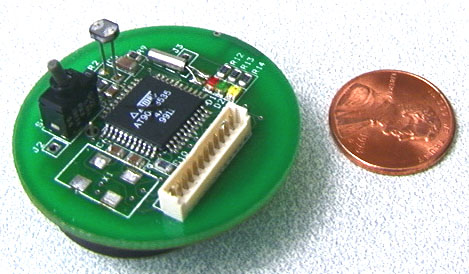
\includegraphics[width=.5\columnwidth]{pics/WeC.png}}
  \caption{WeC Mote}
  \label{fig:WeC}
\end{figure}

In the next years, the 'rene' and 'mica' platforms are developed. In the year 2002, work on the nesC programming language began. Until that, tinyOS consisted of a mixture of C files and Perl scripts. In the same year, tinsOS 1.0, the first tinyOS implemented in nesC, is released. 

Improvement of tinyOS 1.x went on until february 2006, when tinyOS 2.0 beta1 was released. Version 2.1 was finished in april 2007. Among numerous bugfixes, a cc2420 wireless radio stack implementation was added in this release. tinyOS 2.02 was released some months later, which included an cc2420 stack reimplementation and bugfixes.
After that, in august 2008, support for the 'iris' and 'shimmer' platforms was added by distribution of version 2.1. Clearly, bugfixes were included in this release too.

At the time of this writing, the latest tinyOS version is 2.1.1, which was released in April 2010. Most important add-ons are support for the 'mulle', 'epic' and 'shimmer2' - platforms. 

\section{Supported Platforms}

With version 2.1.1, a range of hardware motes are supported out-of-the-box. A brief description of this platforms and its most important communication devices are given in the following list. Obviously, most of this platforms provide interfaces for UART, I2C, SPI or others peripherals, depending of the microcontroller and extension boards used, too. These features are not listed here.

\begin{itemize}
 \item btnode3: Atmega128L cpu and radio/bluetooth communication devices
 \item epic: MSP430 cpu and CC2420 radio chip
 \item eyesIFX: MSP430F149/F1611 and TDA5250 wireless transceiver
 \item intelmote2: PXA271 XScale cpu and CC2420 radio chip 
 \item mica: Atmega103 and TR1000 radio chip
 \item mica2: Atmeage128L and Chipcon 868/916 radio chip
 \item mica2dot: Atmega128 and cc1000 transceiver
 \item micaz: Atmega128 and cc2420 radio chip
 \item mulle: Renesas M16C and AT86RF230 transceiver
 \item sam3s\_ek: SAM3S4C chip and cc2520 transceiver
 \item sam3u\_ek: SAM3S4C chip and cc2420 transceiver
 \item shimmer / shimmer2 / shimmer2r : MSP430 cpu and CC2420 transceiver
 \item span: MSP430 cpu and CC2420 transceiver
 \item telosa / telosb: MSP430 cpu and CC2420 transceiver
 \item tinynode: MSP430 cpu and Semtech SX1211 transceiver
 \item ucmini: Atmega128RFA1 cpu(low power transceiver cpu integrated)
 \item z1: MSP430 cpu and CC2420 transceiver
\end{itemize}

\section{tinyOS hardware abstraction}

When looking at the supported hardware platforms, one can see that many platforms use the same cpu and/or communication hardware. To avoid rewriting of code, hardware abstraction is used.
By introducing hardware abstraction, it is easier to port applications from one platform to another, and application development itself gets easier too. On the other hand, abstraction means generalisation, which is problematic because hardware motes only have very limited resources and strict energy-efficiency requirements.
So, tinyOS uses a 3-level \textit{Hardware Abstraction Architecture} to provide a flexible and performant framework to build applications on, as shown in figure~\ref{fig:haa}.

\begin{figure}[h]
 \centerline{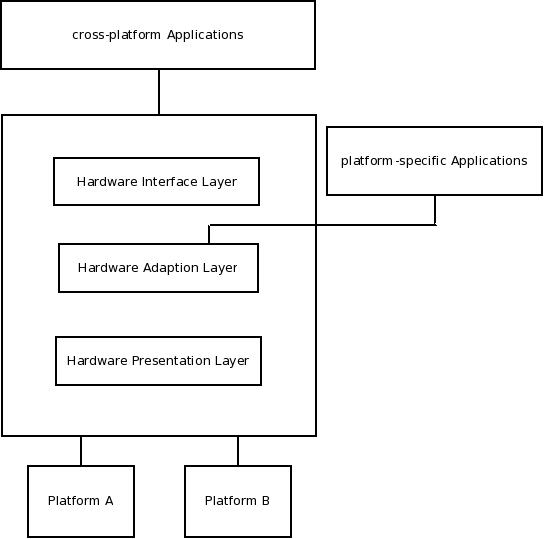
\includegraphics[width=.6\columnwidth]{pics/hardwareabstraction.png}}
  \caption{Hardware Abstraction Architecture}
  \label{fig:haa}
\end{figure}

In contrast to other embedded OS that use only 2 layer abstraction, the third tinyOS layer provides more flexibility. For maximum performance, a \textit{Platform-Specific-Application} can directly hook into the \textit{Hardware Adaption Layer}, circumventing the \textit{Hardware Interface Layer}.


\section{tinyOS internals}

\subsection{Basic - Scheduler}

By default, tinyOS 2.x uses a \textbf{non-preemptive FIFO} scheduler with a maximum of 255 parameterless tasks waiting for execution. A task can only be scheduled once at a time, if periodic execution is needed the task has to re-post itself just before finishing. The scheduler itself consists of an interminable for-loop, that pops ( = executes) one task after the other, in sequence as this tasks got pushed. If no tasks are waiting for execution, the scheduler enters a powersaveing-mode immediatly.

Because the scheduler of tinyOS is implemented as a component it is possible to replace this default FIFO-scheduler with a selfwritten one. See ~\cite{tep106:2003} for details how to implement a selfwritten scheduler.

\subsection{Microcontroller Power Management}

To reduce power consumption, a microcontroller should always run in the lowest power state possible. For example, if you want to run an embedded system that is powered by two AA batteries with a capacitiy of 2.7Ah, for one year, you reach an average of about 1mW of power consumption. Clearly, this can only be achieved by saving energy whenever possible.

As mentioned above, tinyOS enters a low power mode if the task queue is empty. Normally, microcontrollers support a range of low power modes, the ATmega128 - for example - supports up to 6 different power saving modes.
To decide what mode fits best, tinyOS uses the control- and statusregisters to find the proper lowpower-mode.

For example, on a ATmega128-based platform, the cpu-specific powersaving-mode \textit{IDLE} is to be choosen if one or more timer, SPI, UART or I2C are in use. If the ADC-submodule is working, another mode, \textit{ADC Noise Reduction}, is entered. If none of this modules are active and the task queue is empty, the cpu is set to \textit{POWER DOWN}, from which it only can resume by some external interrupts/resets or a SPI address match interrupt.

Because entering powersaving modes always come with wakeup latency, problems can arise if some higher-level hardware modules have timeing constraints if the wakeup latency is too big. To solve this, the powersaving mode, found by examing the control- and statusregisters, can be overridden by a higherlevel module. For example, when going to a sleepmode just befor an alarm of a timer would occur, the wakeup latency could propably cause a miss of this alarm. Therefore, a component can \textit{provide} an interface named \textit{lowestState} that will be called when a powersave mode is requested, and can override the in principle valid powersaveing mode found by looking at the control- and statusregisters.

\subsection{Boot Sequence}

When tinyOS is booting up, it uses 3 interfaces:

\begin{itemize}
 \item Init
 \item Scheduler
 \item Boot
\end{itemize}

\textbf{Init} has one command, called \textit{init()}, that is responsible for initializing hardware components. Initialization must happen sequential, so a component is allowed to use a spin loop when - for example - waiting for an interrupt.
\textbf{Scheduler} is responsible for initializing the task queue.
Finally, \textbf{Boot} signales the completion of the bootup-process to the application.

\subsection{Ressource Arbitration}

One major task of every operating system is the management of available resources, like communication interfaces that are used by different components. tinyOS distinguishes between 3 different kinds of abstractions:

\begin{itemize}
 \item dedicated resources
 \item virtualized resources
 \item shared resources
\end{itemize}

A \textbf{dedicated} resource is a resource which is allocated by one and only one subsystem all the time. Obvious, no sharing policy is needed here. Examples for such resources are counters and interrupts.

\textbf{Virtualized} resources are used by multiple clients through software virtualization. Here, every client interacts like using a dedicated reosource. Because virtualization is done in software, there is no upper bound on the number of clients(apart from memory/efficiency constraints), with all virtualized instances being multiplexed on top of the underlying resource. Clearly, this virtualization 
goes along with cpu-overhead.

For example, this concept is used for timers on ATmega128-based platforms. Every time a new timer is instantiated, tinyOS builds a virtual timer on top of the physical timer 0. 

The \textbf{shared} concept is used for modules that need exclusive access to a resource for some time. An arbiter is responsible for multiplexing between the different clients that want to use the resource. As long as a client \textit{holds} a resource, it has complete access to it. tinyOS arbiters assume that clients are cooperative, that means that a client only acquires a resource when needed, and only holds it as long as needed, releasing it as soon as possible. No concept of preemption is used here, so client B that needs a resource cannot force Client A to release it.  

The arbiter, the centralized place that knows whether a resource is busy or not, is an interface that must be instantiated by every client that wants to use the resource. After that, the client can \textit{request} the resource. The request is queued by the arbiter if the resource is busy. As soon as the resource is available, a special event, \textit{granted}, is signaled to the client, who has now exclusive access to it. It is the client's responsibility to \textit{release} it so soon as possible.
To avoid monopolizing a resource a \textit{request} for a resource is only queued if there is no other request of this client queued yet.


%%
%% = eof =====================================================================
%%

    \cleardoublepage
    %%
%%
%% This file should be edited by user
%%

\chapter{bigAVR6} \label{chapter:bigAVR6}


\section{The Hardware}

\section{Supported Modules}

\subsection{GLCD}

\subsection{MMC}

\subsection{Ethernetboard}

\subsection{LCD 2x16}



%%
%% = eof =====================================================================
%%

    \cleardoublepage
    %%
%%
%% This file should be edited by user
%%

\chapter{buildenv} \label{chapter:buildenv}


\section{Prerequisites}




%%
%% = eof =====================================================================
%%

    \cleardoublepage
    %%
%% Concepts
%%
%% This file should be edited by user
%%

\chapter{Concepts} \label{chapter:concepts}

Usually, this chapter is necessary in order to give an overview on
the \emph{terms} and \emph{concepts} that are required to understand
your work.

\section{Writing Style}

Usually you should not use the first person singular (\emph{I}) in
your text, write \emph{we} instead. As a general recommendation, use
the first person sparsely, sometimes it can be replaced by a phrase
like \emph{This work presents...}.

The indefinite article \textbf{a} is used as \textbf{an} before a
vowel sound - for example \textbf{an} apple, \textbf{an} hour,
\textbf{an} unusual thing, \textbf{an} FPGA (becourse the acronym is
pronouned Ef-Pee-Gee-A), \textbf{an} HIL. Before a consonant sound
represented by a vowel letter \textbf{a} is usual -- for example
\textbf{a} one, \textbf{a} unique thing, \textbf{a} historic
chance\footnote{According to Merriam Webster, both \textbf{a} and
\textbf{an} can be used in writing before unstressed or weakly
stressed syllables with initial h, thus you could also write
\textbf{an} historic chance.}.

\section{Acronyms}

Explain acronyms at their first occurrence in the text. In order to
achieve this consistently, we recommend to use the \texttt{acronym}
package.

A new acronym is then declared by writing
\verb+\newacro{acronym}{expanded name}+. Use the macro
\verb+\ac{acronym}+ as a placeholder for the acronym in the text.

See file \texttt{acronym.tex} for further examples and explanations.

\newacro{GPL}{Gnu Public License}

\section{Figures}

A Figure should always be referenced in the text, as it is the case
with Figure~\ref{fig:example}.

\begin{figure}[h]
 \centerline{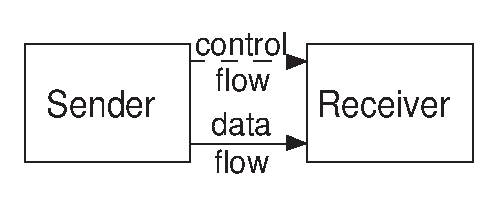
\includegraphics[width=.5\columnwidth]{pics/example}}
  \caption{Example figure}
  \label{fig:example}
\end{figure}

This template can be compiled with the \texttt{latex} command or the
\texttt{pdflatex} command. While \texttt{latex} creates an
intermediate file format (.dvi) that can be further processed into a
\texttt{.ps} or \texttt{.pdf} file, the \texttt{pdflatex} command
directly creates a \texttt{.pdf} file.

Note that with \texttt{latex} the \verb+\includegraphics+ accepts
only .eps files, while with \texttt{pdflatex} accepts \texttt{.pdf},
\texttt{.png}, or \texttt{.jpg}. Luckily, the file extension can be
omitted in order that \verb+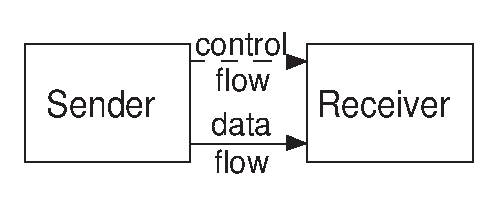
\includegraphics{pics/example}+ will
look for file with name \texttt{example.eps} in \texttt{latex} mode
and for a file with name \texttt{example.pdf}, \texttt{example.png},
or \texttt{example.jpg} in \texttt{pdflatex} mode. If you already
have an \texttt{.eps} file, you may create a respective
\texttt{.pdf} file with the commandline conversion tool
\texttt{epstopdf}.

\section{Citations and References}

Whenever you refer to previously published work, you should set a
reference to acknowledge the work you build upon. For example this
is a reference to two bachelor's theses~\cite{kraut:2003,
weirich:2005}. If you literally cite a part of someone else's work,
mark the respective sentence by quotes and italic letters and add
the page number, where is text can be found:

\dqit{An intelligent or {\em smart} transducer is the integration of
an analog or digital sensor or actuator element, a processing unit,
and a communication interface. In case of a sensor, the smart
transducer transforms the raw sensor signal to a standardized
digital representation, checks and calibrates the signal, and
transmits this digital signal to its users via a standardized
communication protocol.}\cite[p.\,175]{elmenreich:2005}

\section{Spellchecking}

Do not use your advisor as your spell checker. Instead, run an
electronic spell checker over your document before submitting the
document to your advisor.

\section{References with Bibtex}

Bibtex is an additional program to {\LaTeX} that creates a list of
your cited references in a chapter named {\em Bibliography}. In
order to use Bibtex, you must maintain a database of all references
in so-called \emph{bibfiles} (file extension \texttt{.bib}).

The \emph{bibfiles} contain entries of several types, the most
needed types are \texttt{book}, \texttt{inproceedings},
\texttt{article}, \texttt{techreport}, \texttt{mastersthesis}, and
\texttt{phdthesis}. In the following we list the templates for these
types, whereas each asterisk (*) should be replaced by the
respective data, if this is not available, the element should be
left out. The case of the element names does not matter to Bibtex,
however in the examples we have used UPPERCASE for the obligatory
fields and lowercase for the optional fields. To see some complete
examples, have a look into the file \texttt{bibfile.bib}. For more
information, read~\cite{patashnik:1988}.

\subsection{Some BibteX Examples}

\footnotesize
\begin{verbatim}
@BOOK{*,
  AUTHOR =       {*},
  editor =       {*},
  TITLE =        {*},
  PUBLISHER =    {*},
  YEAR =         {*},
  volume =       {*},
  number =       {*},
  series =       {*},
  address =      {*},
  edition =      {*},
  month =        {*},
  note =         {*}
}

@INPROCEEDINGS{*,
  AUTHOR =       {*},
  TITLE =        {*},
  BOOKTITLE =    {*},
  YEAR =         {*},
  editor =       {*},
  volume =       {*},
  number =       {*},
  series =       {*},
  pages =        {*},
  address =      {*},
  month =        {*},
  organization = {*},
  publisher =    {*},
  note =         {*}
}

@ARTICLE{*,
  AUTHOR =       {*},
  TITLE =        {*},
  JOURNAL =      {*},
  YEAR =         {*},
  volume =       {*},
  number =       {*},
  pages =        {*},
  month =        {*},
  note =         {*}
}

@TECHREPORT{*,
  AUTHOR =       {*},
  TITLE =        {*},
  INSTITUTION =  {*},
  YEAR =         {*},
  type =         {*},
  number =       {*},
  address =      {*},
  month =        {*},
  note =         {*}
}

@MASTERSTHESIS{*,
  AUTHOR =       {*},
  TITLE =        {*},
  SCHOOL =       {*},
  YEAR =         {*},
  type =         {*},
  address =      {*},
  month =        {*},
  note =         {*}
}

@PHDTHESIS{*,
  AUTHOR =       {*},
  TITLE =        {*},
  SCHOOL =       {*},
  YEAR =         {*},
  type =         {*},
  address =      {*},
  month =        {*},
  note =         {*},
  abstract =     {*},
  keywords =     {*},
  source =       {*},
} \end{verbatim}




%%
%% = eof =====================================================================
%%

    \cleardoublepage
    %%
%% Related Work
%%
%% This file should be edited by user
%%

\chapter{Related Work} \label{chapter:relatedwork}

This chapter should give an overview over existing work that is
related to your work. Instead of \dq{Related Work}, this chapter can
also be named specifically to the topic of the thesis.

For example in Bernhard Weirich's Bachelor's thesis, there are two
chapters on related work named \dq{Time-Driven Algorithms} and
\dq{Event-Driven Algorithms}~\cite{weirich:2005}.

Each related approach should be described by a section of about
100-500 words.

\section{Types of Bachelor's Theses}

If you write a plain report on some implementation, you might have
no chapter on related works.

%%
%% = eof =====================================================================
%%

    \cleardoublepage
    %%
%% Design Approach
%%
%% This file should be edited by user
%%

\chapter{Design Approach} \label{chapter:designapproach}

If you have derived some new concepts on your own, this is the place
to present them. You can use generic names for this chapter like
\dq{Design Approach} or \dq{System Architecture} or chose name
accordingly to its contents (for example \dq{Automatic Text
Generator Algorithm}).

\section{Types of Bachelor's Theses}

If you write a Bachelor's thesis in form of a survey, you might have
several chapters on existing work from others, but no chapter as
described here.


%%
%% = eof =====================================================================
%%

    \cleardoublepage
    %%
%% Implementation
%%
%% This file should be edited by user
%%

\chapter{Implementation} \label{chapter:implementation}

Call this \dq{Implementation} or \dq{Case Study}, here you will
describe you actual hands-on part of your work.

\section{Types of Bachelor's Theses}

If you write a Bachelor's thesis in form of a survey, you might have
several chapters on existing work in the literature, but no chapter
as described here.


%%
%% = eof =====================================================================
%%

    \cleardoublepage
    %%
%% Results
%%
%% This file should be edited by user
%%

\chapter{Results and Discussion} \label{chapter:results}

Name this chapter \dq{Results and Discussion}, \dq{Experimental
Results}, \dq{Evaluation} or \dq{Experiments and Evaluation}. First
present your measurements here, usually in form of graphs and
tables. Second, discuss it. Explain for example missing or misplaced
data points\footnote{By the way, do not refer to colored elements in
a figure or graph, assume the user prints out your thesis in black
and white}.

If this chapter grows too large, you might split it into two
separate chapters, for example \dq{Results} and \dq{Discussion}.

\section{Tables}

\begin{table}[h]
  \begin{center}
  \begin{tabular}{|l|d{4}|d{4}|d{4}|d{5}@{}|}
    \hline
    Sensor & \multicolumn{1}{C{2.6cm}|}{Mean squar-\\ed error} & \multicolumn{1}{C{2.5cm}|}{Mean abso-\\lute error}
    &  \multicolumn{1}{C{2.5cm}|}{Estimated variance} & \multicolumn{1}{C{2.5cm}|}{Respective confidence} \\
    &  \multicolumn{1}{C{2.6cm}|}{(cm$^2$)} &  \multicolumn{1}{C{2.5cm}|}{(cm)} &
    \multicolumn{1}{C{2.5cm}|}{(cm$^2$)} & \\ \hline \hline
    IR 1 (d $\leq$ 80 cm) & 228.38 & 5.97 & 212.98 & 4\\
    IR 1 (hybrid) & 860.87 & 14.35 & 686.08 & 2\\
    IR 1 (d $>$ 110 cm) & 1880.50 & 28.27 & 1078.30 & 2\\ \hline
    IR 2 (d $\leq$ 80 cm) & 242.04 & 7.25 & 233.15 & 4\\
    IR 2 (hybrid) & 226.04 & 7.15 & 206.56 & 4\\
    IR 2 (d $>$ 110 cm) & 162.13 & 6.24 & 127.92 & 5\\ \hline
    IR 3 (d $\leq$ 80 cm) &  108.45 &  7.35 &  104.82 &  5\\
    IR 3 (hybrid) & 795.57 & 18.59 & 538.91 & 3\\
    IR 3 (d $>$ 110 cm) & 1945.08 & 37.65 & 505.68 & 3\\ \hline
%    US 1 (hybrid) &  25.89 &  2.84 &  25.91 &  7 &\\ \hline
%    US 2 (hybrid) &  8.81 &  1.84 &  8.87 &  8 &\\ \hline
  \end{tabular}
  \end{center}
  \caption{Quality of calibrated infrared sensor data (from~\cite{elmenreich:2002})}\label{table:quality_ir}
\end{table}

Table~\ref{table:quality_ir} shows an example of a table set in
\LaTeX. To be honest, making tables in {\LaTeX} is a complicated and
sumptuous task. A good tutorial about setting tables in {\LaTeX} is
presented bei Axel Reichert in~\cite{reichert:1999} (in German
language).

\section{Types of Bachelor's Theses}

If you write a Bachelor's thesis in form of a survey, you might have
several chapters on existing work in the literature, but no chapter
as described here.



%%
%% = eof =====================================================================
%%

    \cleardoublepage
    %%
%% Conclusion
%%
%% This file should be edited by user
%%

\chapter{Conclusion} \label{chapter:conclusion}

The chapter \dq{Conclusion}, sometimes also named \dq{Summary}
should contain two things:

\emph{Main contribution(s) of this work} -- Why is the world a
better one now ;-)

When you write the conclusion, assume that some quick readers might
not have gone through the whole thesis but are merely peeking into
the conclusion, therefore avoid complicated nomenclature here.

\emph{Outlook} -- what could be the next steps or possible
extensions for this research?

%%
%% = eof =====================================================================
%%

    \cleardoublepage

    \appendix
    \cleardoublepage
    \addcontentsline{toc}{chapter}{Bibliography}
    \bibliography{bibfile}
    \bibliographystyle{alpha}

    %%
%% Setup Guide
%%
%% This file should be edited by user
%%

\chapter{Setup Guide}

You have implemented some system others will use? They will surely
acknowledge a short setup guide here. Describe the system
requirements and setup steps in a precise way here, like for
example:

\section{System Requirements}

In order to use the \emph{thesis template}, you need to install
\LaTeX, furthermore an editor supporting {\LaTeX} is recommended.

\subsection{Required Software for Windows}

For compiling this template, we used the actual version of MikTeX,
which is a an up-to-date implementation of {\TeX} and {\LaTeX} for
all current variants of Windows on x86 systems. MikTeX is freely
available at \url{http://www.miktex.org}.

As an editor, we recommend the free \emph{TeXnicCenter} (available
at \url{http://www.toolscenter.org}). Both, MikTeX and TeXnicCenter
are published under the \ac{GPL}.

\emph{TeXnicCenter} comes with an integrated spell checker,
otherwise you are recommended to install the Windows version of
\emph{aspell}, an open source spell checker under the \ac{GPL},
which is available at \url{http://aspell.net/win32/}.

If also want to do
 grammar checking, try Queequeg
(\url{http://queequeg.sourceforge.net/index-e.html}) or see guides
like the one at
\url{http://www.physics.usyd.edu.au/guides/spell-grammer-latex.html}.

\subsection{Required Software for Linux and BSDs}

The standard distributions for Linux already come with a {\LaTeX}
system (typically \texttt{tetex}).

As an editor, we recommend the Kile editor (available at
\url{http://kile.sourceforge.net/} under \ac{GPL}).

As spell checker we recommend \emph{aspell}, an open source spell
checker that replaces the older \emph{ispell} checker. \emph{aspell}
is included in most distributions, otherwise it can be downloaded
from \url{http://www.gnu.org/software/aspell/}. If also want to do
 grammar checking, try Queequeg
(\url{http://queequeg.sourceforge.net/index-e.html}) or see guides
like the one at
\url{http://www.physics.usyd.edu.au/guides/spell-grammer-latex.html}.

\subsection{Required Software for Apple Mac OS X}

The \emph{darwin ports} (\url{http://darwinports.opendarwin.org/})
provide a port of \emph{teTeX} that can be installed under Apple Mac
OS X.

As an editor, we recommend TeXShop (available at
\url{http://www.uoregon.edu/~koch/texshop/} under \ac{GPL}).

As spell and grammar checker we recommend Excalibur
(\url{http://www.eg.bucknell.edu/~excalibr/}).

\section{Installing the Thesis Template}

The thesis template comes in a zip-archive. Simply extract the
archive into a directory of your choice and start working.

\section{Types of Bachelor's Theses}

Of course, not all Bachelor's theses require a setup guide.

%%
%% = eof =====================================================================
%%

    \cleardoublepage
    %%
%% User Guide
%%
%% This file should be edited by user
%%

\chapter{User Guide}

You have implemented some system others will use? If you were in
their place what kind of documentation would you like to have in
order to start working?

For complex programs, a tutorial that guides the user through a
typical task showing screenshots of the intermediate states is
desirable.

\section{Types of Bachelor's Theses}

Of course, not all Bachelor's theses require a user guide.


\section{How to use the Thesis Template}

\subsection{Files to Edit}

You should edit the following files (unless you remove some of them,
see Section~\ref{section:removingchapters}):

\begin{itemize}
\item \tt title.tex
\item \tt abstract.tex
\item \tt acronyms.tex
\item \tt introduction.tex
\item \tt concepts.tex
\item \tt relatedwork.tex
\item \tt designapproach.tex
\item \tt implementation.tex
\item \tt results.tex
\item \tt conclusion.tex
\item \tt setupguide.tex
\item \tt userguide.tex
\end{itemize}

\subsection{Removing Chapters} \label{section:removingchapters}

Open the file \texttt{thesis.tex} and remove (or insert a comment)
at the lines with the include-commands, for example:

\begin{table}[h]
\begin{center}
\begin{tabular}{|l|l|}
  \hline
  Before & After \\
  \hline
  % after \\: \hline or \cline{col1-col2} \cline{col3-col4} ...
  \verb+%%
%% Concepts
%%
%% This file should be edited by user
%%

\chapter{Concepts} \label{chapter:concepts}

Usually, this chapter is necessary in order to give an overview on
the \emph{terms} and \emph{concepts} that are required to understand
your work.

\section{Writing Style}

Usually you should not use the first person singular (\emph{I}) in
your text, write \emph{we} instead. As a general recommendation, use
the first person sparsely, sometimes it can be replaced by a phrase
like \emph{This work presents...}.

The indefinite article \textbf{a} is used as \textbf{an} before a
vowel sound - for example \textbf{an} apple, \textbf{an} hour,
\textbf{an} unusual thing, \textbf{an} FPGA (becourse the acronym is
pronouned Ef-Pee-Gee-A), \textbf{an} HIL. Before a consonant sound
represented by a vowel letter \textbf{a} is usual -- for example
\textbf{a} one, \textbf{a} unique thing, \textbf{a} historic
chance\footnote{According to Merriam Webster, both \textbf{a} and
\textbf{an} can be used in writing before unstressed or weakly
stressed syllables with initial h, thus you could also write
\textbf{an} historic chance.}.

\section{Acronyms}

Explain acronyms at their first occurrence in the text. In order to
achieve this consistently, we recommend to use the \texttt{acronym}
package.

A new acronym is then declared by writing
\verb+\newacro{acronym}{expanded name}+. Use the macro
\verb+\ac{acronym}+ as a placeholder for the acronym in the text.

See file \texttt{acronym.tex} for further examples and explanations.

\newacro{GPL}{Gnu Public License}

\section{Figures}

A Figure should always be referenced in the text, as it is the case
with Figure~\ref{fig:example}.

\begin{figure}[h]
 \centerline{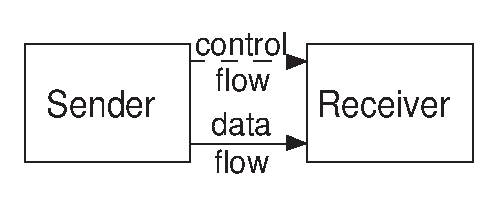
\includegraphics[width=.5\columnwidth]{pics/example}}
  \caption{Example figure}
  \label{fig:example}
\end{figure}

This template can be compiled with the \texttt{latex} command or the
\texttt{pdflatex} command. While \texttt{latex} creates an
intermediate file format (.dvi) that can be further processed into a
\texttt{.ps} or \texttt{.pdf} file, the \texttt{pdflatex} command
directly creates a \texttt{.pdf} file.

Note that with \texttt{latex} the \verb+\includegraphics+ accepts
only .eps files, while with \texttt{pdflatex} accepts \texttt{.pdf},
\texttt{.png}, or \texttt{.jpg}. Luckily, the file extension can be
omitted in order that \verb+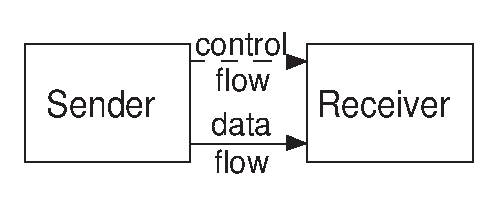
\includegraphics{pics/example}+ will
look for file with name \texttt{example.eps} in \texttt{latex} mode
and for a file with name \texttt{example.pdf}, \texttt{example.png},
or \texttt{example.jpg} in \texttt{pdflatex} mode. If you already
have an \texttt{.eps} file, you may create a respective
\texttt{.pdf} file with the commandline conversion tool
\texttt{epstopdf}.

\section{Citations and References}

Whenever you refer to previously published work, you should set a
reference to acknowledge the work you build upon. For example this
is a reference to two bachelor's theses~\cite{kraut:2003,
weirich:2005}. If you literally cite a part of someone else's work,
mark the respective sentence by quotes and italic letters and add
the page number, where is text can be found:

\dqit{An intelligent or {\em smart} transducer is the integration of
an analog or digital sensor or actuator element, a processing unit,
and a communication interface. In case of a sensor, the smart
transducer transforms the raw sensor signal to a standardized
digital representation, checks and calibrates the signal, and
transmits this digital signal to its users via a standardized
communication protocol.}\cite[p.\,175]{elmenreich:2005}

\section{Spellchecking}

Do not use your advisor as your spell checker. Instead, run an
electronic spell checker over your document before submitting the
document to your advisor.

\section{References with Bibtex}

Bibtex is an additional program to {\LaTeX} that creates a list of
your cited references in a chapter named {\em Bibliography}. In
order to use Bibtex, you must maintain a database of all references
in so-called \emph{bibfiles} (file extension \texttt{.bib}).

The \emph{bibfiles} contain entries of several types, the most
needed types are \texttt{book}, \texttt{inproceedings},
\texttt{article}, \texttt{techreport}, \texttt{mastersthesis}, and
\texttt{phdthesis}. In the following we list the templates for these
types, whereas each asterisk (*) should be replaced by the
respective data, if this is not available, the element should be
left out. The case of the element names does not matter to Bibtex,
however in the examples we have used UPPERCASE for the obligatory
fields and lowercase for the optional fields. To see some complete
examples, have a look into the file \texttt{bibfile.bib}. For more
information, read~\cite{patashnik:1988}.

\subsection{Some BibteX Examples}

\footnotesize
\begin{verbatim}
@BOOK{*,
  AUTHOR =       {*},
  editor =       {*},
  TITLE =        {*},
  PUBLISHER =    {*},
  YEAR =         {*},
  volume =       {*},
  number =       {*},
  series =       {*},
  address =      {*},
  edition =      {*},
  month =        {*},
  note =         {*}
}

@INPROCEEDINGS{*,
  AUTHOR =       {*},
  TITLE =        {*},
  BOOKTITLE =    {*},
  YEAR =         {*},
  editor =       {*},
  volume =       {*},
  number =       {*},
  series =       {*},
  pages =        {*},
  address =      {*},
  month =        {*},
  organization = {*},
  publisher =    {*},
  note =         {*}
}

@ARTICLE{*,
  AUTHOR =       {*},
  TITLE =        {*},
  JOURNAL =      {*},
  YEAR =         {*},
  volume =       {*},
  number =       {*},
  pages =        {*},
  month =        {*},
  note =         {*}
}

@TECHREPORT{*,
  AUTHOR =       {*},
  TITLE =        {*},
  INSTITUTION =  {*},
  YEAR =         {*},
  type =         {*},
  number =       {*},
  address =      {*},
  month =        {*},
  note =         {*}
}

@MASTERSTHESIS{*,
  AUTHOR =       {*},
  TITLE =        {*},
  SCHOOL =       {*},
  YEAR =         {*},
  type =         {*},
  address =      {*},
  month =        {*},
  note =         {*}
}

@PHDTHESIS{*,
  AUTHOR =       {*},
  TITLE =        {*},
  SCHOOL =       {*},
  YEAR =         {*},
  type =         {*},
  address =      {*},
  month =        {*},
  note =         {*},
  abstract =     {*},
  keywords =     {*},
  source =       {*},
} \end{verbatim}




%%
%% = eof =====================================================================
%%
+ & \verb+%%
%% Concepts
%%
%% This file should be edited by user
%%

\chapter{Concepts} \label{chapter:concepts}

Usually, this chapter is necessary in order to give an overview on
the \emph{terms} and \emph{concepts} that are required to understand
your work.

\section{Writing Style}

Usually you should not use the first person singular (\emph{I}) in
your text, write \emph{we} instead. As a general recommendation, use
the first person sparsely, sometimes it can be replaced by a phrase
like \emph{This work presents...}.

The indefinite article \textbf{a} is used as \textbf{an} before a
vowel sound - for example \textbf{an} apple, \textbf{an} hour,
\textbf{an} unusual thing, \textbf{an} FPGA (becourse the acronym is
pronouned Ef-Pee-Gee-A), \textbf{an} HIL. Before a consonant sound
represented by a vowel letter \textbf{a} is usual -- for example
\textbf{a} one, \textbf{a} unique thing, \textbf{a} historic
chance\footnote{According to Merriam Webster, both \textbf{a} and
\textbf{an} can be used in writing before unstressed or weakly
stressed syllables with initial h, thus you could also write
\textbf{an} historic chance.}.

\section{Acronyms}

Explain acronyms at their first occurrence in the text. In order to
achieve this consistently, we recommend to use the \texttt{acronym}
package.

A new acronym is then declared by writing
\verb+\newacro{acronym}{expanded name}+. Use the macro
\verb+\ac{acronym}+ as a placeholder for the acronym in the text.

See file \texttt{acronym.tex} for further examples and explanations.

\newacro{GPL}{Gnu Public License}

\section{Figures}

A Figure should always be referenced in the text, as it is the case
with Figure~\ref{fig:example}.

\begin{figure}[h]
 \centerline{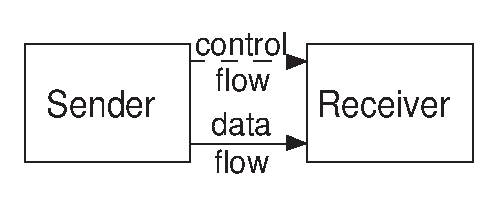
\includegraphics[width=.5\columnwidth]{pics/example}}
  \caption{Example figure}
  \label{fig:example}
\end{figure}

This template can be compiled with the \texttt{latex} command or the
\texttt{pdflatex} command. While \texttt{latex} creates an
intermediate file format (.dvi) that can be further processed into a
\texttt{.ps} or \texttt{.pdf} file, the \texttt{pdflatex} command
directly creates a \texttt{.pdf} file.

Note that with \texttt{latex} the \verb+\includegraphics+ accepts
only .eps files, while with \texttt{pdflatex} accepts \texttt{.pdf},
\texttt{.png}, or \texttt{.jpg}. Luckily, the file extension can be
omitted in order that \verb+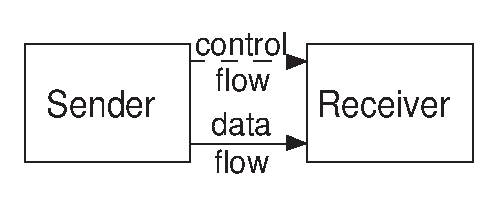
\includegraphics{pics/example}+ will
look for file with name \texttt{example.eps} in \texttt{latex} mode
and for a file with name \texttt{example.pdf}, \texttt{example.png},
or \texttt{example.jpg} in \texttt{pdflatex} mode. If you already
have an \texttt{.eps} file, you may create a respective
\texttt{.pdf} file with the commandline conversion tool
\texttt{epstopdf}.

\section{Citations and References}

Whenever you refer to previously published work, you should set a
reference to acknowledge the work you build upon. For example this
is a reference to two bachelor's theses~\cite{kraut:2003,
weirich:2005}. If you literally cite a part of someone else's work,
mark the respective sentence by quotes and italic letters and add
the page number, where is text can be found:

\dqit{An intelligent or {\em smart} transducer is the integration of
an analog or digital sensor or actuator element, a processing unit,
and a communication interface. In case of a sensor, the smart
transducer transforms the raw sensor signal to a standardized
digital representation, checks and calibrates the signal, and
transmits this digital signal to its users via a standardized
communication protocol.}\cite[p.\,175]{elmenreich:2005}

\section{Spellchecking}

Do not use your advisor as your spell checker. Instead, run an
electronic spell checker over your document before submitting the
document to your advisor.

\section{References with Bibtex}

Bibtex is an additional program to {\LaTeX} that creates a list of
your cited references in a chapter named {\em Bibliography}. In
order to use Bibtex, you must maintain a database of all references
in so-called \emph{bibfiles} (file extension \texttt{.bib}).

The \emph{bibfiles} contain entries of several types, the most
needed types are \texttt{book}, \texttt{inproceedings},
\texttt{article}, \texttt{techreport}, \texttt{mastersthesis}, and
\texttt{phdthesis}. In the following we list the templates for these
types, whereas each asterisk (*) should be replaced by the
respective data, if this is not available, the element should be
left out. The case of the element names does not matter to Bibtex,
however in the examples we have used UPPERCASE for the obligatory
fields and lowercase for the optional fields. To see some complete
examples, have a look into the file \texttt{bibfile.bib}. For more
information, read~\cite{patashnik:1988}.

\subsection{Some BibteX Examples}

\footnotesize
\begin{verbatim}
@BOOK{*,
  AUTHOR =       {*},
  editor =       {*},
  TITLE =        {*},
  PUBLISHER =    {*},
  YEAR =         {*},
  volume =       {*},
  number =       {*},
  series =       {*},
  address =      {*},
  edition =      {*},
  month =        {*},
  note =         {*}
}

@INPROCEEDINGS{*,
  AUTHOR =       {*},
  TITLE =        {*},
  BOOKTITLE =    {*},
  YEAR =         {*},
  editor =       {*},
  volume =       {*},
  number =       {*},
  series =       {*},
  pages =        {*},
  address =      {*},
  month =        {*},
  organization = {*},
  publisher =    {*},
  note =         {*}
}

@ARTICLE{*,
  AUTHOR =       {*},
  TITLE =        {*},
  JOURNAL =      {*},
  YEAR =         {*},
  volume =       {*},
  number =       {*},
  pages =        {*},
  month =        {*},
  note =         {*}
}

@TECHREPORT{*,
  AUTHOR =       {*},
  TITLE =        {*},
  INSTITUTION =  {*},
  YEAR =         {*},
  type =         {*},
  number =       {*},
  address =      {*},
  month =        {*},
  note =         {*}
}

@MASTERSTHESIS{*,
  AUTHOR =       {*},
  TITLE =        {*},
  SCHOOL =       {*},
  YEAR =         {*},
  type =         {*},
  address =      {*},
  month =        {*},
  note =         {*}
}

@PHDTHESIS{*,
  AUTHOR =       {*},
  TITLE =        {*},
  SCHOOL =       {*},
  YEAR =         {*},
  type =         {*},
  address =      {*},
  month =        {*},
  note =         {*},
  abstract =     {*},
  keywords =     {*},
  source =       {*},
} \end{verbatim}




%%
%% = eof =====================================================================
%%
+ \\
  \verb+\cleardoublepage+ & \verb+\cleardoublepage+ \\
  \verb+%%
%% Related Work
%%
%% This file should be edited by user
%%

\chapter{Related Work} \label{chapter:relatedwork}

This chapter should give an overview over existing work that is
related to your work. Instead of \dq{Related Work}, this chapter can
also be named specifically to the topic of the thesis.

For example in Bernhard Weirich's Bachelor's thesis, there are two
chapters on related work named \dq{Time-Driven Algorithms} and
\dq{Event-Driven Algorithms}~\cite{weirich:2005}.

Each related approach should be described by a section of about
100-500 words.

\section{Types of Bachelor's Theses}

If you write a plain report on some implementation, you might have
no chapter on related works.

%%
%% = eof =====================================================================
%%
+ & \verb+%%%
%% Related Work
%%
%% This file should be edited by user
%%

\chapter{Related Work} \label{chapter:relatedwork}

This chapter should give an overview over existing work that is
related to your work. Instead of \dq{Related Work}, this chapter can
also be named specifically to the topic of the thesis.

For example in Bernhard Weirich's Bachelor's thesis, there are two
chapters on related work named \dq{Time-Driven Algorithms} and
\dq{Event-Driven Algorithms}~\cite{weirich:2005}.

Each related approach should be described by a section of about
100-500 words.

\section{Types of Bachelor's Theses}

If you write a plain report on some implementation, you might have
no chapter on related works.

%%
%% = eof =====================================================================
%%
+ \\
  \verb+\cleardoublepage+ & \verb+%\cleardoublepage+ \\
  \verb+%%
%% Design Approach
%%
%% This file should be edited by user
%%

\chapter{Design Approach} \label{chapter:designapproach}

If you have derived some new concepts on your own, this is the place
to present them. You can use generic names for this chapter like
\dq{Design Approach} or \dq{System Architecture} or chose name
accordingly to its contents (for example \dq{Automatic Text
Generator Algorithm}).

\section{Types of Bachelor's Theses}

If you write a Bachelor's thesis in form of a survey, you might have
several chapters on existing work from others, but no chapter as
described here.


%%
%% = eof =====================================================================
%%
+ & \verb+%%
%% Design Approach
%%
%% This file should be edited by user
%%

\chapter{Design Approach} \label{chapter:designapproach}

If you have derived some new concepts on your own, this is the place
to present them. You can use generic names for this chapter like
\dq{Design Approach} or \dq{System Architecture} or chose name
accordingly to its contents (for example \dq{Automatic Text
Generator Algorithm}).

\section{Types of Bachelor's Theses}

If you write a Bachelor's thesis in form of a survey, you might have
several chapters on existing work from others, but no chapter as
described here.


%%
%% = eof =====================================================================
%%
+ \\
  \verb+\cleardoublepage+ & \verb+\cleardoublepage+ \\
  \hline
\end{tabular}
\end{center}
  \caption{Removing the Chapter \texttt{Related Work}}\label{table:removing}
\end{table}

\subsection{Adding Chapters} \label{section:addingchapters}

Open the file \texttt{thesis.tex} and add an
\verb+\include{+\emph{filename}\verb+}+ command (followed by a
\verb+\cleardoublepage+) at the respective line. Then create a new
file \emph{filename}\verb+.tex+ in the same directory and write the
chapter's contents into it.

\subsection{Adding References} \label{section:addingreferences}

Whenever you \verb+\cite+ something, there must be a respective
entry in any of the included .bib files. To add such an entry, open
the respective bibfile (\eg \texttt{bibfile.bib}) with a text editor
and add the entry according to the bibfile syntax. The reference
will be added after running latex/bibtex/latex on your project.

\subsection{Removing References} \label{section:removingreferences}

Remove all \verb+\cite+ commands to this reference in the text and
the citation will not be listed in the bibliography after running
latex/bibtex/latex on your project. There is no need to remove the
reference from the .bib file.

\subsection{Changing the .bib Files to be used}

In the file \texttt{thesis.tex} there is a line with a
\verb+\bibliography+ command, that lists all used .bib files without
file extensions separated by commas.

\subsection{Troubleshooting}

If you make something wrong, you should get an error at compile
time, except for citation problems, like:

\begin{description}
\item[Adding or removing references does not work:]~~Perhaps there is
a spelling error in some .bib file, this causes the program
\texttt{bibtex} to abort execution leaving the old bibliography
unchanged.

\item[Changing a reference does not work:]~~Some systems only perform
a new bibtex run if there are missing references, delete the
\texttt{.aux} file in order to overcome this problem.

\item[References show a question mark:]~~Bibtex could not find a
matching entry in the bibfile for this reference, check the label
name.

\end{description}



%%
%% = eof =====================================================================
%%

    \cleardoublepage

\end{document}

%%
%% = eof =====================================================================
%%
